\documentclass[letterpaper]{article}
\usepackage{amsmath}
\usepackage{algorithm}
\usepackage{multirow}
\usepackage{graphicx}

\begin{document}
\title{ECON 199 Problem Set 1}
\author{Will Koster (jameswk2)}
\author{Javier Garza (javierg2)}
\date{Feb 25, 2020}
\maketitle

\clearpage

\section{Problem 1}
\begin{enumerate}
    \item 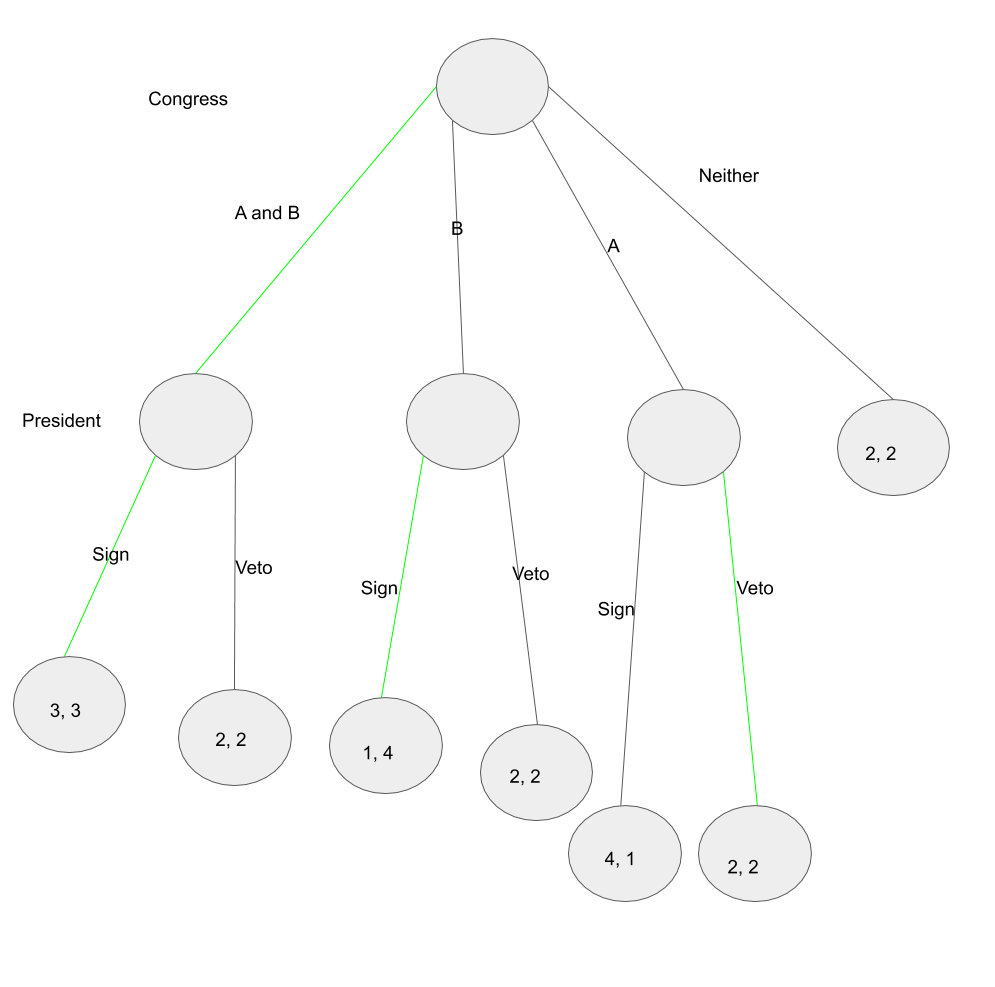
\includegraphics[scale=0.4]{fig1}
    \item 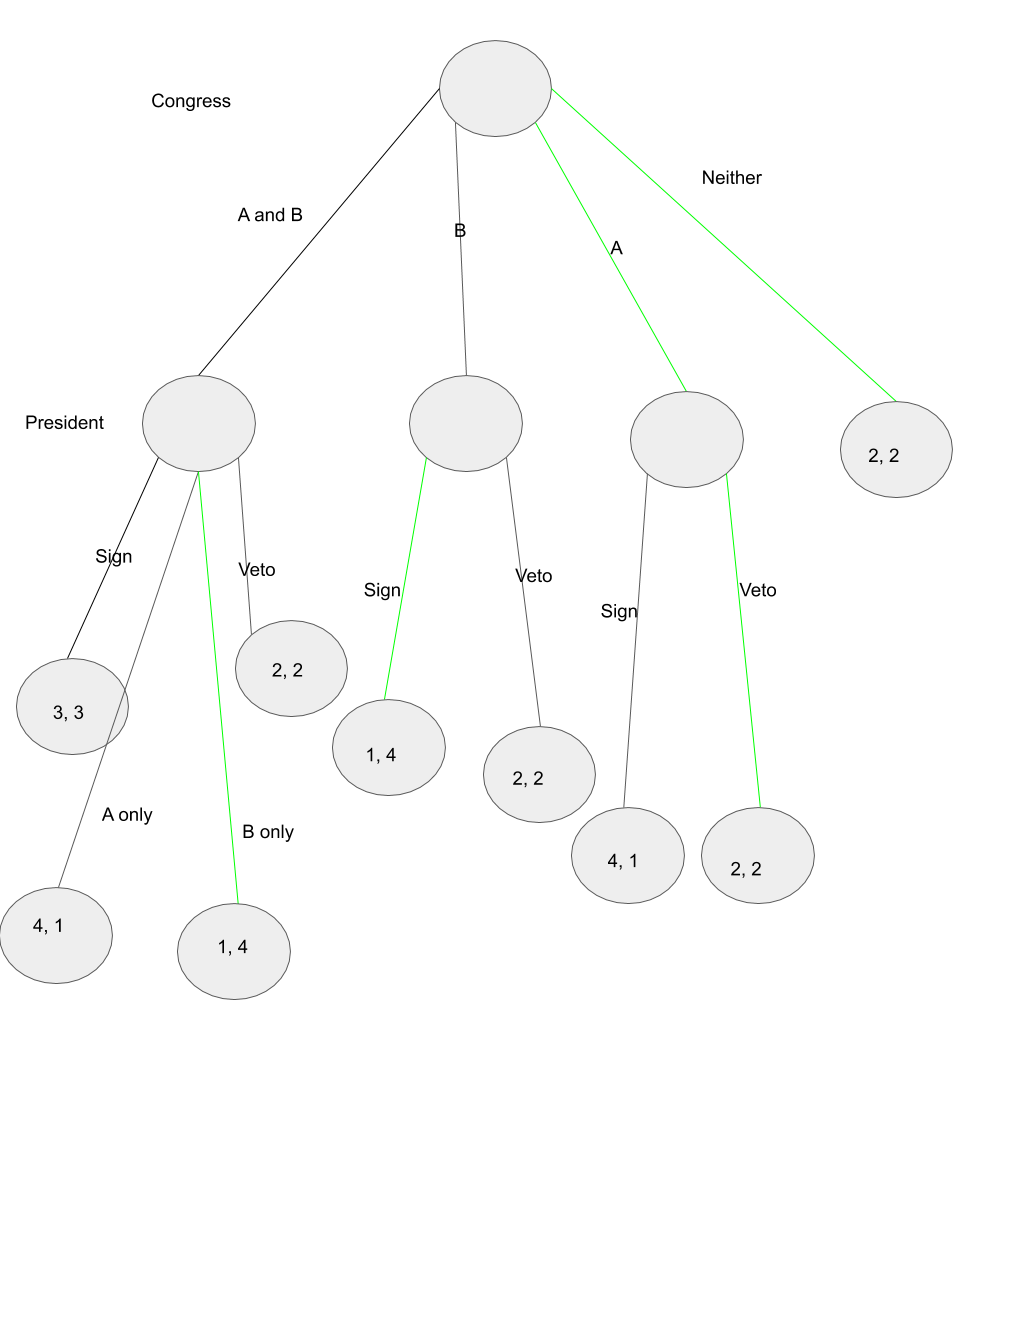
\includegraphics[scale=0.4]{fig2}
    \item In the first situation, Congress could force the President to give it something in exchange for giving the President what he wanted, but in the second situation, that was no longer the case, so Congress no longer had any incentive to give the President anything.
\end{enumerate}

\section{Problem 2}
\begin{enumerate}
    \item 
David Buys \\
\begin{tabular}{|l|l|l|l|}
\multicolumn{4}{c}{Colleen}                      \\ \hline
\multirow{3}{*}{Bruce} &   & B        & N        \\ \hline
                       & B & $10,10,10$ & $\overline{10},\overline{20},\overline{10}$ \\ \hline
                       & N & $\overline{20},\overline{10},\overline{10}$ & $0,0,-10$ \\ \hline
\end{tabular} \\
David does not buy \\
\begin{tabular}{|l|l|l|l|}
\multicolumn{4}{c}{Colleen}                      \\ \hline
\multirow{3}{*}{Bruce} &   & B        & N        \\ \hline
                       & B & $\overline{10},\overline{10},\overline{20}$ & $-10,0,0$  \\ \hline
                       & N & $0,-10,0$ & $\overline{0},\overline{0},\overline{0}$ \\ \hline
\end{tabular}\\

\item The Nash equilibria are when any two people buy shshi or none of them do.  
\item Unless there were some situation that is not captured in the game (eg David lives next door to the sushi place, Colleen is the wealthiest, etc), we would have to assume that every member of the group makes the same independent decision. In that case, the focal point would likely be that no one buys sushi, since, under the assumption that your friends do the same thing, it's always optimal for you to not buy sushi, reglardless of what they both choose to do.
\end{enumerate}
\section{Problem 3}

\end{document}
